% Template ripped from:
% http://www.cs.technion.ac.il/~yogi/Courses/CS-Scientific-Writing/examples/simple/simple.htm


\date{\today}

\documentclass[12pt]{article}

\usepackage{graphicx}
\usepackage{listings}
\usepackage{idrislang}
\usepackage{amsfonts,amsthm,amsmath}
\usepackage[en,nat,farve,titelside]{ku-forside}

\newtheorem{defn}{Definition}[section]

\opgave{M.Sc. Thesis}
\forfatter{
        Casper Holmgreen and Knut Liest\o l
        % going by alphabetical order here....
}
\title{Differential Privacy with Dependent Types}
\undertitel{or: How I Learned to Stop Worrying and Love Dependent Types}
% TODO 2 : make a catchy subtitle
\vejleder{Ken Friis Larsen}
\dato{November 11, 2015}


\begin{document}
\maketitle

\lstset{language=idris,
basicstyle=\footnotesize,
frame=single,
numbers=left,
breaklines=true,
postbreak=\raisebox{0ex}[0ex][0ex]{\ensuremath{\color{red}\hookrightarrow\space}}
}

\graphicspath{{assets/}}
\begin{abstract}
This is the paper's abstract \ldots
\end{abstract}

% TODO 1 : write an abstract
% TODO 2 : add captions and labels to all code snippets

\section{Introduction}\label{sec:introduction}

With each passing day, more and more of our personal information is being collected, cataloged and analyzed by an ever increasing number of interested parties.
Their interests range from selective marketing of products and services to collecting business performance metrics and even to malicious and potentially illegal surveillance.
We don't curate and control the data they are collecting;
in many ways, the data we produce actually gives a better picture of who we are than any data we might try to curate and control.
Therefore, as the producers of this data, we should be concerned with how it is being used.

Our medical records consist of very personal information which we reasonably expect to remain private.
Many countries even require legal privacy guarantees for systems maintaining sensitive information, e.g. the Health Insurance Portability and Acountability Act (HIPAA) in the USA.
However, our medical records contain valuable information for researchers aiming to understand health trends in our society.

The benefits of ubiquitous data are not limited to medicine, either.
``Big Data'' is a hot buzzword right now and for good reason: almost everything we do is being quantified and recorded.
Imagine the potential insights we as a society could discover about ourselves with unlimited access to all of our own data.
We are faced with a classic balancing act: how do we protect the privacy of the individual while maximizing the usefulness of our data?

Differential privacy\cite{journals/cacm/Dwork11} is an emerging field aiming to answer this question.
One of the key ideas in differential privacy is that of indistinguishability, i.e. a query against a dataset should return more-or-less the same result regardless of whether or not Alice's records are included in the data.
If the results are indistinguishable, with or without Alice's data, then the contents of her records must be indistinguishable, too.

Indistinguishability is achieved by combining the true (distinguishable) result of a query with random noise.
However, the addition of noise is insufficient by itself to guarantee privacy.
A malicious data analyst could repeat semantically equivalent queries and compute the average of the results, eventually approaching the true mean as he runs more and more queries.
How can this be prevented?
By imposing a hard limit on how many queries can be run against a data set.
Another key idea in differential privacy is that of the privacy ``budget''.
The privacy budget is a value which limits the number of queries that can be run against a particular data set.
Each query has a cost associated with it which is subtracted from the budget when it is evaluated.
The data set is destroyed when the privacy budget is depleted.

Many algorithms and metrics have been developed by the differential privacy community.
Each algorithm is typically bundled with some sort of proof that it meets some privacy constraints or has some other privacy-related properties.
The burden of producing such a proof and algorithm is typically manual, and therefore error-prone.

PINQ\cite{conf/sigmod/McSherry09} is a differential privacy framework that takes a different approach.
It is a SQL-like query domain specific language (DSL) for the Microsoft .NET languages which guarantees differential privacy by construction.
Users of PINQ are able to compose carefully implemented primitives to build differentially private computations.
The composition of these primitives happens according to well-defined rules, allowing PINQ to track privacy metrics as users build complex differentially private algorithms.
A trusted runtime-system tracks and rejects queries whose cost exceed the remaining privacy budget.

PINQ and its trusted system manage the budget at runtime.
An analyst has no way of knowing whether a query will be accepted without manually tracking their budget.
Reed and Pierce\cite{conf/icfp/ReedP10} solve this by building a strongly-typed programming language which represents query costs in the types.
% TODO 3 : Include more about DFuzz to lead into our hypothesis?
We aim to build on this idea by demonstrating that a dependent type system is a natural fit for capturing differential privacy requirements.

Strongly-typed programming languages are capable of statically verifying programs for type-correctness, precluding many potential sources of runtime errors: ``well-typed programs can't go wrong''.
We extend this notion of being ``well-typed'' to include differential privacy metrics.
Just as PINQ is embedded in the .NET languages (particularly C\#), we plan to embed our implementation within the dependently-typed, functional programming language: Idris\footnote{http://idris-lang.org}.
This allows us to take advantage of Idris' parser and advanced type checker, as well as the many improvements continually being made by Idris' active open-source community.

Well-typed programs in our embedded language can't go wrong and also can't violate their privacy requirements.
Formal proofs for type-correct algorithms written in our language are unnecessary - the program itself is the proof.
Thus, all type-correct programs must respect expected privacy constraints.

\subsection{Contributions}

This paper describes an implementation of an embedded prototype language, \texttt{DPDT}, for describing differentially private computations.
Dependent type systems have come a long way since Martin-L\"of's original intuitionistic type theory.
We show that dependent types are a natural fit for describing and verifying differential privacy constraints.

We implemented a fully-typed abstract language for describing the relational algebra; and we developed a simple in-memory Idris database backend for it.
% TODO 3 : include reference to Power of Pi paper again?
Our main contribution is the layering of differential privacy metrics into the types over top of the fully-typed relational algebra.
PINQ's differential privacy metrics are checked dynamically at runtime, whereas our privacy layer leverages the power of dependent types to verify that privacy constraints are not violated \textit{at compile time}.

% TODO 1 : add more contributions if there are any

\paragraph{Outline}

In Chapter~\ref{sec:differential_privacy}, we cover some necessary background for understanding the basics of differential privacy.
Chapter~\ref{sec:dependent_types_in_idris} serves as a brief tutorial to Idris with a focus on the language features we make use of in our implementation.
Chapter~\ref{sec:function_sensitivity} combines the contents of the previous two chapters in an example implementation of function sensitivity.
Chapter~\ref{sec:typing_the_relational_algebra} reviews the relational algebra and how we represent it using dependent types.
Chapter~\ref{sec:our_implementation} covers the differential privacy layer that we built over top of the fully-typed relational algebra.
We evaluate our work in Chapter~\ref{sec:evaluation} and provide concluding remarks in Chapter~\ref{sec:conclusion}.

\section{Differential Privacy}\label{sec:differential_privacy}

In this section, we describe some of the central ideas and metrics behind differential privacy.
We begin by motivating the necessity for differential privacy before moving on to outlining the key concepts used in our implementation.

% TODO 1 : first part of this section and Intro overlap a lot!

In today's Big Data world, more and more of our data is being stored on servers belonging to others.
Even though it may feel like it, we are not the consumers of free online services: we are the product.
But regardless of whether we freely volunteered it, were legally compelled to share it, or just bought something online, we have a reasonable expectation to privacy of our data.

However, databases containing large amounts of personal data can be tremendously valuable for researchers looking into a variety of important questions.
For example, epidemiologists may be able to detect and prevent the spread of disease and doctors may be able to monitor and/or analyze the long-term health trends of a large population over time.
Big Data offers us huge potential for learning about ourselves, but most of these databases are held under lock and key.
How to best balance database utility with individual privacy is the question differential privacy aims to answer.

Many approaches have been devised for sharing data while respecting privacy.
One approach, which has made news headlines a few times by now (not in a positive light), is to anonymize or otherwise ``fuzz'' a dataset before releasing it to the public.
However, it has quickly become evident that it is not possible to release a database that is both accurate enough to be useful and that respects the privacy of the participants\cite{journals/cacm/Dwork11}.

Differential privacy aims to maximize database utility while minimizing the risk for all individuals contained within.
Traditionally, privacy research has focused on preventing a malicious attacker from learning anything about a particular individual (e.g. our dear friend Alice).
However, this has proved to be nearly impossible in the presence of auxiliary information. ((WHY))
% TODO 2 : why?
% TODO 2 : talk about the parallel to cryptography guarantees

Rather than trying to prove the impossibility of a privacy breach, differential privacy guarantees that a users participation in a database can only increase their risk of a privacy breach by a negligible amount.
This is true regardless of how much auxiliary information a would-be attacker knows or might learn in the future.

Analysts are able to run differentially private algorithms against private data knowing that no individuals' privacy can be compromised.
Suddenly, many of the Big Data databases which would otherwise be off limits can be made available to researchers.
Each individuals participation in the database has a negligible effect on their risk of a privacy breach, so honest participation follows as a direct consequence.

In fact, a classic example of differentially private thinking is randomized response.
Randomized response is a technique originally proposed in 1965 for encouraging survey respondents to answer potentially embarassing questions honestly.
By introducing an element of randomness, participants are given plausible deniability regardless of how they respond.

After reading the question, participants are instructed to flip a coin.
If the coin yields ``tails,'' the participant responds ``No''.
If the coin reads ``heads,'' he/she answers truthfully.
The net result is that $1/2$ of the responses are ``No'' by default, while the other half should be a representative sampling of the population.
Thus, if researchers using randomized response find that 10\% of participants admit to an illegal activity, the true percentage is actually around 20\%.

% TODO 1 : outline the metrics to come

The rest of this section will focus on specific ideas from the differential privacy literature as it relates to our implementation of DPDT.
In particular, we will discuss function sensitivity, which is a relative measure of how much a function can magnify the distances between collections of objects; and indistinguishability, which is the key idea which quantifies what it means for a computation to be differentially private.
Finally, we describe PINQ, the framework that allows users to build differentially private computations by construction.

\subsection{Function Sensitivity}
% TODO 1 : this section overlaps with chapter on function sensitivity

Function sensitivity is an important concept from the differential privacy literature.
We can make assertions about an entire program if we understand the sensitivities of the functions with which it is composed.
Sensitivity is a key part in making our type system work.

Function sensitivity captures the idea of how relatively ``far'' a function can magnify the distances between pairs of objects.
We say that a function is $c$-sensitive if, for all pairs of inputs, the distance between the outputs does not exceed $c$ times the original distance between the inputs.

\begin{defn}\label{def:csens}
  A function, $f : \mathbb A \rightarrow \mathbb A$, is $c$-sensitive if
  $$\forall x,y.\; d_{\mathbb A}(f(x),f(y)) \le c \times d_{\mathbb A}(x,y)$$
\end{defn}

For a concrete example, let us turn our attention to the domain of real numbers.
We will take the distance function to be $d_\mathbb{R}(x,y) = |x - y|$.
Obviously, the function $f_{id}(x)=x$ cannot magnify distances at all.
For any two real numbers, their difference will equal the difference between them after applying $f_{id}$.

\[
  \forall x,y.\; d_\mathbb{R}(f_{id}(x),f_{id}(y)) = d_\mathbb{R}(x,y)
\]

We say $f_{id}$ is 1-sensitive because distances can't be magnified at all.
Another example of a 1-sensitive function is $f_{1/2}(x) = x/2$; in fact, $f_{1/2}$ is also $\frac{1}{2}$-sensitive.

\begin{defn}\label{def:clessthancprime}
  A function that is $c$-sensitive is also $c'$-sensitive for all $c < c'$.
\end{defn}

Similarly, consider the case where $f_{+10}(x) = x + 10$.
Clearly, it doesn't matter which $x$ and $y$ you sample; the distance $d_{\mathbb R}(x,y)$ will always equal $d_{\mathbb R}(f(x),f(y))$.
Therefore, $f_{+10}$ is a 1-sensitive function.
Now consider the case of $f_{\times 2+10}(x) = 2x + 10$.
Distances between input and output objects can be now be doubled (but no more), so it is a 2-sensitive function.
Intuitively, when dealing with linear functions on $\mathbb R$ and the absolute value norm, the largest linear coefficient will dictate the c-sensitivity.
Higher order polynomials are necessarily $\infty$-sensitive.

\begin{figure}
    \centering
    \def\svgwidth{\columnwidth}
    \input{assets/RealDistances.pdf_tex}
    \caption{Real distances and sensitivities}
\end{figure}

Simple functions on $\mathbb R$ and one dimensional distance functions are not terribly interesting.
However, function sensitivity can be applied much more generally and to much more interesting domains, such as databases containing sensitive information (e.g. Alice's tax records or health information).

We will use $\mathbb D$ to describe the domain of all possible databases.
Hence, a function $f : \mathbb D \rightarrow \mathbb D$ is an endomorphism for databases.
The distance between two databases is their symmetric difference; i.e. $d_{\mathbb D}(D_1,D_2) = | D_1 \oplus D_2 |$.
There is a special case that turns up often in the differential privacy literature.
We are primarily concerned with whether a particular individual's records are included in the database or not.

\begin{defn}
  We denote the case when two databases, $D_1$ and $D_2$, differ by exactly 1 row (i.e. $d_{\mathbb D}(D_1,D_2)=1$) with the special notation: $D_1 \sim D_2$.
\end{defn}

Despite the change of scenery, function sensitivity behaves as outlined above.
Consider a database endomorphism, $filter_p : \mathbb D \rightarrow \mathbb D$, which filters rows according to some pre-specified predicate, $p$.
$filter_p$ is a 1-sensitive function because adding Alice's in the database adds at most one row to the result for all possible values of $p$.

For all pairs of databases, $D_1$ and $D_2$, the distance between them is $d_{in} = d_{\mathbb D}(D_1,D_2)$.
The distance $d_{out} = d_{\mathbb D}(filter_p(D_1),filter_p(D_2))$ cannot exceed $d_{in}$.
$filter_p$ will only remove rows from a database, so we have only to consider the possible cases.
There are three main cases to consider:
1) the filter removes a row that is in both of the databases,
2) the filter removes a row that is in exactly one of the databases, and
3) the filter removes a row that is in neither of the databases (does nothing).

\paragraph{Case: the filter removes a row that is in both of the databases.}
Because the row is included in both of the input databases, their symmetric difference is unaffected by its presence.
The row is in neither of the output databases, so their symmetric difference is also unaffected.
Therefore, after the removal of the one row, $d_{out} = d_{in}$.

\paragraph{Case: the filter removes a row that is in exactly one of the databases.}
The symmetric difference of the input databases is affected by this row, because it is in one, but not the other.
Therefore, this row is increasing the distance between the input databases.
Its removal brings the output databases closer together.
Therefore, $d_{out} < d_{in}$.

\paragraph{Case: the filter removes a row that is in neither of the databases.}
This is nearly the same as the first case.
The output distance is equal to the input distance.

\paragraph{} % to get a blank line between last P and this one
In all cases, $d_{out}$ is either less than or equal to $d_{in}$.
Thus, we can fix $c=1$ and conclude that filtering is a 1-sensitive function.

Similar proofs exist for the other relational algebra operators.
Proofs like these provide the basic building blocks used by PINQ and DPDT.
The real power of PINQ and DPDT, however, comes from the ability to freely combine these building blocks without having to manually consider sensitivies.

Consider two functions, $f : \mathbb D \rightarrow \mathbb D$ and $g : \mathbb D \rightarrow \mathbb D$, with sensitivities $c$ and $c'$, respectively.
What is the sensitivity of the function resulting from their composition, $k = f . g$?
Function sensitivities compose multiplicatively; i.e. $k$ is $(c\times c')$-sensitive.
Sensitivity represents the largest factor by which the distances between pairs of objects can be increased, so it follows that the composition of sensitivities is multiplicative.

\subsection{Indistinguishability}

Indistinguishability is the key idea that distinguishes differential privacy from similar approaches in privacy research.
If an attacker is unable to determine whether Alice's data even exists in the database, he will be unable to determine the contents of her data.
A query is said to be differentially private if it satisfies this property.

We turn to randomness to achieve this kind of behavior.
Consider a randomized function, $f_r : A \rightarrow B$.
Then, for all $x,y \in A$, if the probability of both $f_r(x)$ and $f_r(y)$ being in $S \subseteq B$ is nearly equal, then it is nearly impossible to determine which input was used.
% TODO 3 : clarify what $S$ is in this case

$$ Pr[f_r(x)\in S] \qquad\approx\qquad  Pr[f_r(y)\in S] $$

This is the core idea behind indistinguishability.
The intrinsic randomness of the function prevents an attacker from deducing anything about the input based on the output.
Now consider a randomized query, or mechanism, $\mathcal M(D) : \mathbb D \rightarrow \mathbb R$.
We say that such a query is $\epsilon$-differentially-private if the inclusion of Alice's data affects her privacy risk by at most $e^\epsilon$. % TODO 4 : What is 'privacy risk'

\begin{defn}\label{def:diffpriv}
  A randomized mechanism, $\mathcal{M}(D) : \mathbb D \rightarrow A$, is $\epsilon$-differentially-private if, for all databases $D_1 \sim D_2$, and all $S \in A$,
  $$Pr[\mathcal M(D_1)\in S] \le e^\epsilon \times Pr[\mathcal M(D_2)\in S]$$
\end{defn}
% TODO 1 : check whether S \in R should be \in or \subseteq

% TODO 1 : discuss how to use noise
% TODO 1 : discuss aggregations
There are a few restrictions on mechanisms in the context of sensitive databases.
Obviously, there are limits to the types of data that queries are allowed to return.
We can't allow entire tables (computed or otherwise) to be returned, because they will potentially contain the sensitive rows we are trying to protect!
Additionally, queries should not be allowed to return data directly from any particular row.

In fact, queries must be restricted to aggregation operations.
This may seem limiting, but in practice is not so.
Certainly, entire classes of queries and algorithms are precluded by this necessity, but the vast majority of statistical research is performed using aggregations over tables, not querying for the information pertaining to particular individuals.

An additional constraint emerges from the previous one: the data type returned by the aggregation must be a semigroup; i.e. it must have an associative binary operator for folding new values into the aggregate.
However, aggregations alone are not capable of protecting privacy.

Consider a database consisting of all patients who have ever been treated at the \textit{ABC ABortion Clinic}.
Alice is one of those patients.
Regardless of what Alice's records actually contain, her mere presence in that database could have serious consequences for her private life if the wrong people found out.
Consider the result of the following query: \textit{How many people named Alice are in the database?}
One.
That is a valid aggregation and Alice is now in trouble.

So how could we have saved Alice?
The final requirement is randomness.
When we run an aggregation, we need to randomize the output to satisfy indistinguishability.
If not, an attacker can draft clever aggregations to deduce private information about particular individuals.
Noising the result before returning it gives Alice plausible deniability.
The aggregation function from earlier will no longer be enough to determine whether any records in the database related to Alice and what they contain if they do.

Generally, the Laplace distribution is used because XX.
% TODO 1 : why do we prefer Laplace? it scales well with e and is symmetric. what else?

\subsection{PINQ}\label{sec:pinq}

This section provides an overview of PINQ, the framework we modelled our language after.
PINQ is a privacy layer built over top of the .NET query DSL LINQ.
% TODO 3 : expand on what LINQ is to make PINQ's contribution more clear?
It provides carefully implemented primitives and the ability to build arbitrarily complex, differentially private algorithms from them.
There are two main components to PINQ: transformations and aggregations.
Each PINQ server will keep track of its own privacy budget and reject queries whose costs exceed the remaining budget.
Once a data source's budget is entirely consumed, it will be impossible to query it again through the PINQ interface.

\subsubsection{Transformations}

LINQ is a query DSL written for the .NET languages allowing users to manipulate data with relational algebra operators directly in the host language.
In LINQ terminology, these operations are called transformations.
Our work includes a fully-typed LINQ-like implementation in Idris (\texttt{Database.PowerOfPi.Idris}).

PINQ's big contribution is the addition of a privacy layer around LINQ.
Most of LINQ's transformations are still available in the PINQ API.
% TODO 4 : which ones aren't and why
However, they have all been carefully reimplemented to keep track of their function sensitivities.
Each transformation is aware of its own sensitivity and the sensitivies of the subqueries beneath it.
The word ``stability'' is commonly used when discussing sensitivity in the context of database transformations.
We have already seen a proof that a filtering function (selection) is 1-sensitive.
Similar proofs exist for all of the other transformations provided by PINQ.

% TODO 1 : figure out what to do with the rest of this subsection

\texttt{select} is a projection and will return the same number of rows as the input, and thus removing a particular row in the input will remove exactly one row and affect no other row of the result.

\texttt{where} is a selection and will return a subset of the input rows.
If we remove one of the input rows, the change in the result will be at most one row.

\texttt{groupBy} is an example of a 2-stable transformation.
This is because removing one row of the input can potentially both remove a group and the member in this group, leading to a symmetric difference of 2.

\subsubsection{Aggregations}

As shown earlier, the only safe way to return data from a sensitive database is through aggregations.
PINQ provides a few carefully implemented aggregation operations and disallows everything else.
Each aggregation is proven to be $\epsilon$-differentially private.
$\epsilon$ is an argument provided by the user to specify how much of the privacy budget should be consumed to run the aggregation.
The ultimate cost of a query is the product of the transformation stability and $\epsilon$.
The more costly a query is, the more accurate the result may be.

The simplest of PINQ's mechanisms is \texttt{noisyCount}, which just returns the number of rows described by the given query plus some noise.
\texttt{noisyCount} is a 1-sensitive function.
Consider two databases which differ by exactly one row, $D_1 \sim D_2$.
Because we know the databases differ by only one row, the distance between the inputs is $d_{\mathbb D}(D_1,D_2)=1$.
Similarly, we know that the counts of the two databases must differ by one; i.e. $d_{\mathbb R}(noisyCount(D_1),noisyCount(D_2))=1$.
% TODO 1 : fix the line breaking issue here
We can fix $c=1$ and conclude that \texttt{noisyCount} is a 1-sensitive function.
\texttt{noisyCount} is made $\epsilon$-differentially private by adding Laplacian noise scaled according to $1/\epsilon$.
% TODO 3 : add \qed after each ``proof''?

Another aggregation mechanism PINQ provides is \texttt{noisyAverage}.
This aggregation adds a unique challenge with regards to function sensitivity.
Let us assume that we have a function, $r : \texttt{Row} \rightarrow \mathbb R$.
$r$ yields a numeric value for each row and we want to compute the average value of all the rows contained in the query.
Let $f : \mathbb D \rightarrow \mathbb R$ be the aggregation function which maps $r$ onto all rows and reduces them to their average (i.e. $f = \texttt{average . map r}$).
What is $f$'s sensitivity?

Consider the pair of databases $D_1 \sim D_2$.
Just as before, the distance between them is 1.
How much of an effect can that one row have on the distance between the output averages?
It is impossible to say with the information we have now.

Imagine a database containing the ages of students at a particular university.
In the United States, their ages will most likely range from 18 to 22.
For illustrative purposes, let us assume that $trueAverage(D_1) = 20$.
Alice, who just turned 40 and is having a mid-life crisis, has decided to go back to college.
How will her participation in the database affect $trueAverage(D_2)$?

It depends on how many students already attend the college.
Let's say it is a small college of just one prior student.
Alice's participation has brought $trueAverage(D_2) = 30$!
College of 20,000?
$trueAverage(D_2) = 20.000999$.
And we had to assume that we knew Alice's age to get this far!
In reality, we will have no idea what outlier values $r$ might yield.
We are unable to quantify the effect of that one row on the aggregate.
Thus, we must conclude that $trueAverage$ is $\infty$-sensitive.

PINQ solves this by making \texttt{noisyAverage} clamp values to the range $[-1,+1]$.
In doing so, PINQ is able to conclude that no row is able to affect the aggregate by more than 2.
Then we can add noise scaled according to $2/\epsilon$.
What if $trueAverage(D) + Lap(2/\epsilon)$ falls outside of the specified range?

PINQ solves this by looping over new noise values until the constraint is satisfied.
We improve on this behavior by noting that the Laplace cumulative distribution function (CDF), which is used to sample from the Laplace distribution, is invertible.
We usually use a uniform random variable sampled from the interval $[0,1)$ to draw from the Laplace distribution.
Our implementation computes the subinterval for the uniform random variable that guarantees the constraint will be met.

% TODO 2 : make a figure of the invertible CDF?

Of course, the decision to clamp values to the interval $[-1,+1]$ will require analysts to pre-process their data.
This will require users to explicitly express their assumptions regarding the range of possible values that $r$ could return.
If we wanted to compute the average age of the college students from before, we might draft an invertible function mapping the interval $[18,22]$ to $[-1,+1]$.
Then, if we get a response of $0$, we can translate that back to $20$.

% TODO 4 : talk about more aggregations? Or at least mention them
% TODO 4 : find another way to close this chapter out solidly

\section{Dependent Types in Idris}\label{sec:dependent_types_in_idris}

Idris is a general purpose pure functional programming language with dependent types.
Dependent types allow types to be predicated on values.
With this feature, larger portions of a program can be descibed in types, and can thus be verified by the compiler.

This section will serve as a introduction to dependent types in Idris, but will not describe the language in whole.
Familiarity with a functional programming language is a pre-requisite.
First we will have a look at how basic dependent types work in Idris, then we will introduce some features used later in this report.

A simple example of a good fit for a dependent type is a list with a fixed length, namely a vector.
Here the vector type is \textit{indexed} by a natural number representing the length. 
In other words, a vector type is dependent on a length. 
In addition, like a list, the vector type is \textit{parameterized} by the item type.
A type that is indexed by a value is called a type family.

\begin{lstlisting}
|||Vector type signature in Idris
data Vect : (length:Nat) -> (itemType:Type) -> Type
\end{lstlisting}

Using the vector as an example, we can create some functions on vectors in which the types reflect the functionality. As illustrated in the example above, types are first class language constructs in Idris. A type has the type \textit{Type} and can be passed around a program and computed as any other type.

\begin{lstlisting}
append : Vect n a -> Vect m a -> Vect (n + m) a

reverse : Vect n a -> Vect n a

take : (n : Nat) -> Vect (n + m) a -> Vect n a
\end{lstlisting}

Notice how the signature of append in itself makes it fairly clear what the function does.
Not only is it useful to users to see descriptive signatures like these, but it proves very helpful during implementation.
The Idris compiler will complain if the returned data type does not match the defined return type.
This excludes a lot of possible implementation errors, which in turn reduce the amount of unit tests needed to validate the functionality.

\subsection{Construction}

\begin{lstlisting}
data Nat = Z | S Nat 
\end{lstlisting}

Data types are constructed using a syntax similar to that of Haskell\footnote{https://www.haskell.org/}.
The data type above represents natural numbers recursively.
There are two constructors, $Z$ and $S$ $Nat$.
$Z$ constructs a zero and $S$ $n$ constructs the successor of $n$.

\begin{lstlisting}
data Vect : Nat -> Type -> Type where
   Nil  : Vect Z a
   (::) : a -> Vect k a -> Vect (S k) a
\end{lstlisting}

Type families like Vect have to provide a value for a index during construction, so the constructor syntax is a bit more complex than the one of Nat.

\subsection{Operator sections}

In addition to named functions, Idris has support for anonymous functions.
Anonymous functions, also called lambda abstractions, can be used to provide the implementation of a function on the fly, without having to make a named one.

\begin{lstlisting}
||| Anonymous id fn
\x => x

||| Anonymous integer add fn
\x, y => x + y

\end{lstlisting}

Idris also provides constructs for writing anonymous functions more compactly, namely operator sections.
$(*2)$ is a operator section that simply multiplies a numeric value by 2.
It expands to \lstinline{\x => x * 2}, and can be passed into functions and applied to a numeric argument.

\subsection{Monad and do-notation}

In functional programming, a Monad is a structure that abstracts away some computation.
It defines how to chain Monad instances together, such that users don't have to be concerned with the abstracted computations.

An example of a Monad instance is the state monad. 
Pure functional languages don't have global state or mutable variables.
In order to represent state in a pure language an immutable state construct can be passed explicitly into functions that need state.
We then update the state by constructing a new state based on the old state.

% TODO 3: Add more complex example for motivation
\begin{lstlisting}
addToState : Int -> Int -> Int
addToState x state = x + state
\end{lstlisting}

Passing the state explicitly works fine for a simple example as above, but leads to a lot of boilerplate code if the repeated computations are complex.
The state monad abstracts away the state operations, so users can access the state if needed with less boilerplate.

In Idris, Monad is a typeclass, which is an abstract class.
An example of an instance of the Monad typeclass is the state monad.

Idris provides a do-notation for sequentially interacting with monad instances in a clean manner.

\begin{lstlisting}
addToState : Int -> State Int Int
addToState x = do
   	state <- get
        return (x + state)
\end{lstlisting}

The do-notation allows us to get the state out of the monad context, perform computations on it, and return the updated state.
In Idris a data type can get access to do-notation by implementing the chaining function \lstinline{>>=} and the \lstinline{return} function.

\subsection{Implicit arguments and automatic proof search}

Even though Idris' type checker is rather powerful, there is still correct types that can not be validated by the type checker alone.
The \lstinline{head} function on a list is an example of such a type.
\lstinline{head} returns the first element of the list.
By providing a static proof that the list is not empty, the implementation below is correct.

\begin{lstlisting}
head : (xs : List a) -> (isCons xs = True) -> a
head (x :: xs) _ = x
\end{lstlisting}

Idris also allows function arguments to be implicit, meaning that it is not necessary to pass the argument in during function application.
This is a good fit for proofs, like \lstinline{isCons} for \lstinline{head}.

\begin{lstlisting}
head : (xs : List a) -> {auto p : isCons xs = True} -> a
head (x :: xs) = x
\end{lstlisting}

Implicit arguments are written in curly braces, and can be derived in different ways, one being the automatic proof search.
Automatic proof search is invoked by adding the \lstinline{auto} annotation to an implicit argument, and makes Idris search for a matching type.
If it can't find a matching type, the proof has to be passed in explicitly, or the program will not compile.

Too access an implicit argument within a function, the parameter name is surrounded by curly braces as illustrated by $p$ below.

\begin{lstlisting}
head : (xs : List a) -> {auto p : isCons xs = True} -> a
head (x :: xs) {p} = x
\end{lstlisting}




Concepts used later in the paper that need to be defined here:

\begin{itemize}
\item Idris data constructors cannot share names with type constructors
\item Very small segment about sections (e.g. \texttt{(*10)})
\item do-notation overloading, even without Monad instance
\item Syntax sugar rules
\item Auto proofs
\item TBD
\end{itemize}

\section{Function Sensitivity in Idris}\label{sec:function_sensitivity}

This section demonstrate how we use dependent types to model function sensitivity in Idris.

Modelling function sensitivity with dependent types is fairly straight-forward.
In fact, using Idris it is quite simple.
Recall that function sensitivity is a metric describing how much a function can amplify the distances between pairs of objects.

$$ \forall x,y.\; d(f(x),f(y)) \le c \times d(x,y) $$

We want to reflect the sensitivity of the function in its type, so we will need to index the type on some numeric value.
To keep this example simple, we will use \texttt{Float} to represent sensitivity, but our implementation uses an implementation of \texttt{Rational}s, which should be more stable numerically than IEEE floating point numbers.

We define a type constructor indexed by the sensitivity and parameterized by its input and output types.
It has just one data constructor which is used for wrapping native Idris functions.
A \texttt{SensitiveFunction s a b} is a function with sensitivity \texttt{s} mapping from \texttt{a} to \texttt{b}.

\begin{lstlisting}
||| Represents a sensitive function
||| @ c The sensitivity of the function
||| @ a The input type of the function
||| @ b The output type of the function
data SensitiveFunction : (c:Float) -> (a:Type) -> (b:Type) -> Type where
    MkSensitiveFunction : (a -> b) -> SensitiveFunction s a b

namespace Examples

    add10 : SensitiveFunction 1 Float Float
    add10 = MkSensitiveFunction (+10)

    doubleThenAdd10 : SensitiveFunction 2 Float Float
    doubleThenAdd10 = MkSensitiveFunction (*2)

    cheat : SensitiveFunction 1 Float Float
    cheat = MkSensitiveFunction (*20)
\end{lstlisting}

Notice the \texttt{cheat} example above.
It is possible to define sensitive functions which intentionally misrepresent their sensitivities.
Our focus here is not on the verification of a function's sensitivity, but rather on the interaction between sensitivity and the type system under operations such as function composition or application.
Unrestricted application is as simple as unwrapping the function and applying it to an argument.
Function composition returns a new type indexed by the combined sensitivies of the underlying functions.
This is done simply by wrapping the composed functions in a new data constructor and letting the types work out the rest.

\begin{lstlisting}
||| Applies a sensitive function to an input
||| @ f The sensitive function be apply
||| @ x The input
apply : (f:SensitiveFunction s a b) -> (x:a) -> b
apply (MkSensitiveFunction f) x = f x

||| Composes two sensitive functions
||| @ g The outer function
||| @ f The inner function
(.) : (g:SensitiveFunction s b c) -> (f:SensitiveFunction s' a b) -> SensitiveFunction (s*s') a c
(.) (MkSensitiveFunction g) (MkSensitiveFunction f) = MkSensitiveFunction (g . f)
\end{lstlisting}

Now we are able to compose sensitive functions and Idris' type-checker will understand the resulting sensitivities.
See Listing~\ref{lst:composition_examples} for examples of how the type-checker verifies sensitivities.

\begin{lstlisting}[caption={Examples of Sensitive Function Composition},label={lst:composition_examples}]
doSomeMath : SensitiveFunction 2 Float Float
doSomeMath = add10 . doubleThenAdd10

--doesNotCompile : SensitiveFunction 4 Float Float
--doesNotCompile = add10 . doubleThenAdd10

doSomeMath2 : SensitiveFunction ?sens Float Float
doSomeMath2 = add10 . doubleThenAdd10
\end{lstlisting}

One unfortunate consequence of having such a powerful type-system is that all top-level names must have an associated type declaration.
This means that despite the fact that the type-system is capable of computing the costs, we must still explicitly provide the function sensitivity in the type declaration (as in the \texttt{doSomeMath} signature above).
Because the computation is decidable, users will be able to ask Idris for help through its interactive proof search feature.
Asking Idris to find a proof of the hole \texttt{?sens} will yield \texttt{fromInteger 2}.

\section{Typing the Relational Algebra}\label{sec:typing_the_relational_algebra}

In this section, we review the relational algebra and show how it can be modelled in a dependently typed language.
Our approach is based on \cite{OurySwierstra08PowerOfPi}.
% TODO 3 : make this sentence citation read better

The relational algebra describes semantics for modelling and querying data in relational databases (e.g. MySQL\footnote{https://www.mysql.com/}).
E.F. Codd described relational databases and their associated algebra back in the 1970's\cite{codd70}.
The relational model quickly became popular for its simplicity and good performance.

Tables are the fundamental objects which relations build on.
The rows of a table represent individual entities and the columns represent their attributes.
Each of these columns is associated with a data type.
Every table has a \textit{schema}, which is a list of its column names and their types.
For example, the Table~\ref{tab:people_table} contains four columns; each has a unique name and an associated data type.

\begin{table}[tb]
    \caption{People Table}
    \label{tab:people_table}
    \centering

    \begin{tabular}{|c|c|c|c|}
    \hline

    \hline
    \textbf{Key} & \textbf{Name} & \textbf{Age} & \textbf{FavoriteFood} \\
    \hline
    \textit{Int} & \textit{String} & \textit{Int} & \textit{String} \\
    \hline
    \hline
       1 & Casper & 26 & Rogan Josh Curry \\
       2 & Knut & 26 & Moussaka \\
    \hline

    \end{tabular}
\end{table}

The relational algebra allows us to build structured queries against relational databases.
The primary operators are listed below.
Note that some of the operators may require expressions to be provided (e.g. for filtering a table with a conditional).

\begin{itemize}
    \item selection
    \item projection
    \item Cartesian product\footnote{\label{fn:set_ops} These operations function identically to their set counterparts, but impose additional requirements regarding table schemas. In particular, union and difference (and therefore intersection) require that the schemas of the two operands match. The Cartesian product operator requires that the two schemas are disjoint.}
    \item set union\footnotemark[\ref{fn:set_ops}]
    \item set difference\footnotemark[\ref{fn:set_ops}]
\end{itemize}

Note that the set operations and Cartesian product impose additional requirements in this context.
These extra constraints have precluded many type systems from being able to fully type-check the relational algebra.
Strongly-typed languages, such as Haskell, have devised clever solutions to this problem, but none are as straight-forward as the approach available to a dependent type system.
The ability to capture schemas directly in the types and to manipulate them yields a deceptively simple, but powerful typing framework for relational databases.

\subsection{Relational Algebra in Idris}

This section will briefly outline a basic implementation of the relational algebra in Idris.
We begin by defining some simple algebraic datatypes (ADTs) for keeping the types clear.
We then define a toy expression language before moving on to the query language.

First, we need to be able to represent table attributes (columns).
An \texttt{Attribute} is just the pairing of a name (\texttt{String}) to a data type.
Following David Christiansen's lead, we opt to use \texttt{(:::)} instead of the more traditional \texttt{(,)} for constructing our pairs.
% TODO 1 : add reference to D.C.'s implementation of SQLite type providers
We believe this enhances readability of long \texttt{Schema}s, which are just lists of \texttt{Attribute}s.

\begin{lstlisting}
||| Represents an attribute
data Attribute : Type where
  (:::) : String -> Type -> Attribute

||| Represents a schema
Schema : Type
Schema = List Attribute

namespace Examples

    people : Schema
    people = [ "Key"          ::: Int 
             , "Name"         ::: String
             , "Age"          ::: Int
             , "FavoriteFood" ::: String
             ]
\end{lstlisting}

The relational algebra assumes the existence of an expression language, so we implement a primitive one for demonstration.
An expression has access to all of a row's attributes during evaluation and can return a value of any type.
So we index expression types by their \texttt{Schema} and parameterize them by the return type.
Thus, an expression with the type \texttt{Expr s a} can be read as an expression with access to the attributes in schema \texttt{s} returning type \texttt{a}.
Notice that we have not yet defined any underlying representation for the rows.

Expressions are built up from other expressions, forming an expression tree.
See Figure~\ref{fig:expr_tree} for an example of a simple expression tree.

\begin{figure}[h!]
    \centering
    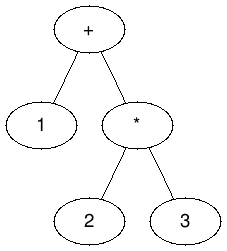
\includegraphics[width=0.25\linewidth]{assets/expr_tree.png}
    \caption{Example Expression Tree $(1 + 2 \times 3)$}
    \label{fig:expr_tree}
\end{figure}
% TODO : resize and work with this graph. write about it in the neighboring text

The return type of the tree in Figure~\ref{fig:expr_tree} is obvious, but what type will a more complex tree from our expression langage have?
Expressions cannot change the schema, so that must remain constant even as the tree grows.
The root of the tree represents the last ``operation'' to be evaluated.
The value returned by this node will be returned, therefore the return type of the root of the tree is the return type of the entire tree.
The type-checker is capable of verifying the types throughout the entire tree, so only well-typed expressions are allowed by the type-system.

\begin{lstlisting}
||| Represents an abstract expression indexed by its schema
||| @ s The schema available to the expression
||| @ a The return type of the expression
data Expr : (s:Schema) -> (a:Type) -> Type where
  ||| Represents a literal value
  Lit    : t -> Expr s t
  ||| Look up a value in the schema
  (^)    : (s:Schema) -> (nm:String) -> { auto p : (map cast s) `ContainsKey` nm } -> Expr s (lookupType s p)
  ||| Represents addition
  (+)    : Num t => Expr s t -> Expr s t -> Expr s t
  ||| Represents equality check
  (==)   : Eq t  => Expr s t -> Expr s t -> Expr s Bool
  ||| Lifts a pure Idris function into the expression language
  PureFn : (a -> b) -> Expr s a -> Expr s b

namespace Examples

  fountain_of_youth : Expr people Int
  fountain_of_youth = people^"Age" - 10

  -- doesNotCompile : Expr people Int
  -- doesNotCompile = people^"DNE"
\end{lstlisting}

In fact, the type-system is even aware when we try to reference columns that don't exist.
Remember, we haven't even mentioned a backend yet; all of this safety is coming exclusively from the type-system.

One of PINQ's neat features is that users have access to nearly all of the features of the host language.
The \texttt{PureFn} data constructor lifts pure Idris functions into the expression language, which should allow clever developers to bend even this simple expression language into something quite powerful.
This functionality is only available to the Idris backend.

\texttt{ContainsKey} is a proof that the given schema contains the attribute in question.
It is derived automatically, so users of our language should never have to worry about it.
\texttt{lookupType} is able to use this proof to statically verify the types.

The core of the relational algebra consists of the query operators, which we model as follows.
\texttt{Query} is implemented as a data family, allowing us to adjust its internal data representation just enough to implement a variety of backends.
In particular, the representation of tables is very backend specific.
For example, an in-memory Idris backend might store pointers directly to the tables in memory, whereas a SQL backend might just store the name of the table as a string.
One of the benefits of this is that any dataset which can be modelled using the relational algebra is usable.

\begin{lstlisting}
mutual -- required for mutual definitions

  ||| Represents an abstract query
  ||| @ t A function yielding a base table representation given a schema
  ||| @ s The schema of the query
  data Query : (t:Schema -> Type) -> (s:Schema) -> Type where
    Table   :       t s -> Query t s
    Union   : Query t s -> Query t s -> Query t s
    Diff    : Query t s -> Query t s -> Query t s
    Product : Query t s -> Query t s' -> { auto p : Disjoint s s' } -> Query t (s ++ s')
    Projection : (f:String -> Maybe String) -> Query t s -> Query t (projectedSchema f s)
    Select  : Expr s Bool -> Query t s -> Query t s

  ||| Represents an abstract grouping
  ||| @ t A function yielding a base table representation given a schema
  ||| @ s The schema of the query
  ||| @ k The type of the grouping key
  data Grouping : (t:Schema -> Type) -> (s:Schema) -> (k:Type) -> Type where
    GroupBy : Eq k => Expr s k -> Query t s -> Grouping t s k

  ||| Represents an abstract partitioning
  ||| @ t A function yielding a base table representation given a schema
  ||| @ s The schema of the query
  ||| @ k The type of the partitioning key
  data Partitioning : (t:Schema -> Type) -> (s:Schema) -> (k:Type) -> Type where
    Partition : Eq k => List k -> Expr s k -> Query t s -> Partitioning t s k

namespace Examples

  -- Tables in our Idris backend are: List (Row s)
  IdrisBackend : Schema -> Type
  IdrisBackend s = List (Row s)

  -- Tables in our SQLite backend are represented by their names
  SQLiteBackend : Schema -> Type
  SQLiteBackend _ = String
\end{lstlisting}

Recall that the set operators require additional constraints that less powerful type systems have a difficult time capturing.
Set union and difference require that the two operands share matching schemas.
Cartesian product requires that they be disjoint.
Notice how easily type unification allows us to express the first two constraints.
The disjoint proof is only slightly more complex; but because it is decidable it can be automatically derived, so the users will be unaware of any additional complexity.

% TODO : write about backends

In trying to emulate PINQ, we chose to focus most of our efforts on implementing an in-memory Idris backend.
However, we believe that our abstract representation of the relational algebra allows for a wide variety of backends to be developed.
The exception to this is \texttt{PureFn}, which is only available to Idris-based backends (e.g. an Idris-based server a la LINQ providers).
Many uses of \texttt{PureFn} could be replaced by extensions to the expression language.

There are two main components required to make a functioning backend implementation:
1) an underlying data representation and
2) evaluator functions that understand our abstract expression and query trees.
Existing database systems such as \texttt{MySQL}\footnote{https://www.mysql.com/} and \texttt{SQLite}\footnote{https://sqlite.org/} already have their underlying data representations.
Implementing backends for them would likely require compiling abstract syntax trees down to SQL strings which could then be submitted to the database.

Our Idris backend uses a basic \texttt{cons}-list structure indexed over \texttt{Schema}s.
Listing~\ref{lst:idris_backend} shows this.
It also shows snippets from expression and query evaluation functions written for Idris and SQLite backends, respectively.

\begin{lstlisting}[caption={Backend Implementation Snippets},label={lst:idris_backend}]
||| Represents a row of data in memory
||| @ s The row's schema
data Row : (s:Schema) -> Type where
  Nil  : Row []
  (::) : Eq t => t -> Row s -> Row (name:::t::s)

namespace IdrisBackend
  ||| Evaluates an abstract expression in the Idris backend
  evalE : Expr s t -> Row s -> t
  evalE (x + y) r = eval x r + eval y r
    [..]

  ||| Evaluates an abstract query in the Idris backend
  evalQ : (q:Query Table s) -> Table s
  evalQ (Product x y) = [ x' ++ y' | x' <- eval x, y' <- eval y ]
    [..]

namespace SQLiteBackend
  ||| Compiles an abstract expression to a SQLite string
  evalE : Expr s t -> String
  evalE (x + y) = "(" ++ eval x ++ ") + ("  ++ eval y ++ ")"
    [..]

  ||| Compiles an abstract query to a SQLite string
  evalQ : Query SQLiteTable s -> String
  evalQ (Product x y)    = "(" ++ eval x ++ ") , (" ++ eval y ++ ")"
    [..]
\end{lstlisting}

\section{Our implementation}\label{sec:our_implementation}

In this section, we describe how we bring together the material of the previous chapters and outline our entire implementation.

Our goal is to leverage Idris's type-checker to statically verify differential privacy constraints.
We create new types to capture the necessities.
We will focus on \texttt{PINQuery} because the other two have similar implementations, but are case-specific.

\begin{lstlisting}
||| Represents an abstract, stability-aware query
||| @ t A function yielding a base table representation given a schema
||| @ s The schema of the query
||| @ c The stability of the query
data PINQuery : (t:Schema -> Type) -> (s:Schema) -> (c:Stability) -> Type where
    MkPINQuery : Query t s -> PINQuery t s c

||| Represents an abstract, stability-aware grouping
||| @ t A function yielding a base table representation given a schema
||| @ s The schema of the query
||| @ k The type of the grouping key
||| @ c The stability of the query
data PINGrouping : (t:Schema -> Type) -> (s:Schema) -> (k:Type) -> (c:Stability) -> Type where
    MkPINGrouping : Grouping t s k -> PINGrouping t s k c

||| Represents an abstract, stability-aware partitioning
||| @ t A function yielding a base table representation given a schema
||| @ s The schema of the query
||| @ k The type of the partitioning key
||| @ c The stability of the query
data PINPartitioning : (t:Schema -> Type) -> (s:Schema) -> (k:Type) -> (c:Stability) -> Type where
    MkPINPartitioning : Partitioning t s k -> PINPartitioning t s k c
\end{lstlisting}

A \texttt{PINQuery t s c} describes a \texttt{c}-differentially private query with schema \texttt{s} (and backend table representation \texttt{(t s)}).
There is only one data constructor which serves simply to wrap a \texttt{Query}, which was defined in Section~\ref{sec:typing_the_relational_algebra}.
This allows us to define a \texttt{Query} and assign it an arbitrary stability.

Next, we provide the standard operators from the relational algebra.
Instead, we unwrap the \texttt{Query} and then rewrap it in the same data constructor, but using a different type constructor.
This is because the schema and stability could potentially change.
We control the API that is exported, so we carefully implement the relational algebra operators with the correct stability costs.
By unwrapping and rewrapping the \texttt{Query} trees from Section~\ref{sec:typing_the_relational_algebra} in our new type, we are now able to build query trees that carry privacy metrics in the type.

\begin{lstlisting}
||| Represents stability-aware selection
where' : PINQuery b s c -> Expr s Bool -> PINQuery b s c
where' (MkPINQuery q) e = MkPINQuery (Select e q)

||| Represents stability-aware projection
select : PINQuery b s c -> (f:String -> Maybe  String) -> PINQuery b (projectedSchema f s) c
select (MkPINQuery q) f = MkPINQuery (Projection f q)

||| Represents stability-aware union
union : PINQuery b s c -> PINQuery b s c' -> PINQuery b s (c + c')
union (MkPINQuery q) (MkPINQuery q') = MkPINQuery (Union q q')

||| Represents stability-aware intersection
intersect : PINQuery b s c -> PINQuery b s c' -> PINQuery b s (c + c')
intersect (MkPINQuery q) (MkPINQuery q') = MkPINQuery (Diff q q')

||| Represents stability-aware grouping
groupBy : Eq k => Expr s k -> PINQuery b s c -> PINGrouping b s k (c * 2)
groupBy e (MkPINQuery q) = MkPINGrouping (GroupBy e q)
\end{lstlisting}

\texttt{where'} is a 1-sensitive function and it's type declaration reflects that.
% TODO 2 : reference proof of filter from earlier
The \texttt{c} parameter remains unchanged through the rewrapping.

\texttt{union}, however, costs the sum of the costs of the operands.
Notice how easily this is described in Idris.

Of course, we can't just return the results of any query.
A query might just return the database contents untouched, potentially violating every single participant's privacy.
Differential privacy essentially requires that any query response be the result of some sort of aggregation.

Additionally, the control flow of a program may be predicated on the value returned from an aggregation.
Sequential queries are additive in cost.
Sequencing computations in functional programming is traditionally accomplished using the infamous \texttt{Monad}.
In many languages, Idris included, types implementing \texttt{Monad} instances have access to special syntactic sugar, commonly known as \texttt{do}-notation.
It is important to note that \texttt{do}-notation is not magic!
It just allows developers an alternative method for writing monadic code.

We want to take advantage of this, but the type signatures required to satisfy a monad instance preclude our ability to reflect sensitivities in the types.
Fortunately, Idris does not actually require a \texttt{Monad} instance to overload \texttt{do}-notation.
We just need to provide the functions \texttt{(>>=)} and \texttt{return}.

\begin{lstlisting}
||| Represents a differentially private computation
||| @ c The privacy cost of the computation
||| @ a The return type of the computation
data Private : (c:Sensitivity) -> (a:Type) -> Type
    MkPrivate : (CrapGen -> (a,CrapGen)) -> Private budget a

||| Lifts a value into a private computation
return : a -> Private 0 a
return x = MkPrivate $ \s => (x,s)

||| Sequences two private computations
(>>=) : Private s a -> (a -> Private s' b) -> Private (s + s') b
(>>=) (MkPrivate sf) f = MkPrivate $ \st => let (x,st1)       = sf st
                                                MkPrivate sf' = f x
                                             in sf' st1

||| Evaluates a private computation
evalPrivate : Private s a -> CrapGen -> a
evalPrivate (MkPrivate f) g = fst (f g)

namespace Examples

    nestedAggregations : Private 3 Double
    nestedAggregations = do x <- the (Private 1 Double) someAggregation
                            y <- the (Private 2 Double) someOtherAggr
                            return ((x+y*2)/3)
\end{lstlisting}

Experienced functional programmers will probably recognize that \texttt{Private} is functionally equivalent to a \texttt{State} monad instance.
Laplace noise requires pseudorandom number generation, so we are keeping track of a generator throughout the computation.

Each aggregation is responsible for providing differential privacy.
Our implementation provides several common aggregations, such as \texttt{noisyCount} and \texttt{noisyAverage}.
Experts will be able to write their own aggregations to provide to the public.

Of course, aggregation alone is not sufficient for guaranteeing privacy.
We must add Laplace noise according to the sensitivity of the \texttt{PINQuery} and a user-provided epsilon.

\texttt{noisyCount} is a good example of a simple aggregation.
The user provides a \texttt{PINQuery} (which has an associated stability cost) and an arbitrary epsilon reflecting how accurate they want the result to be.
The added noise is scaled according to the user provided epsilon while the privacy cost of the entire computation is computed in the types.

\begin{lstlisting}
||| Differentially private mechanism for counting the
||| number of rows described by a query for the Idris backend
||| @ q The query
||| @ e User provided epsilon, accuracy parameter
noisyCount : (q:PINQuery IdrisTable s c) -> (e:Epsilon) -> Private (c*e) Double
noisyCount (MkPINQuery q) eps = MkPrivate $ \g => 
  let (rx,g') = rndDouble g
      noise   = samplePure 0 (1 / toFloat eps) rx
      count   = the Double $ fromInteger $ fromNat $ length (eval q)
   in (count + noise, g')
\end{lstlisting}

\section{Evaluation}\label{sec:evaluation}

In this section, we will evaluate how well dependent types allow differential privacy metrics to be tracked and verified in the type system.
We begin our evaluation of DPDT with simple queries before moving on to more complex algorithms.
% TODO 3 : does this section actually do that?

\subsection{Differentially private queries}

We begin by verifying the behavior of DPDT with simple queries.
There are enough moving parts in a differentially private mechanism to warrant this.
Listing~\ref{lst:example_data_people} constructs a small database in our Idris backend.

\begin{lstlisting}[caption={Example Data},label={lst:example_data_people}]
import Database.PowerOfPi.Idris

Person : Schema
Person = [ "Name" ::: String , "Age" ::: Double ]

people : PINQuery IdrisTable Person 1
people = MkPINQuery $ Table [ [ "Alice"  , 40 ]
                            , [ "Casper" , 26 ]
                            , [ "Knut"   , 26 ]
                            , [ "Tor"    , 26 ]
                            , [ "Gismo"  ,  2 ]
                            ]
\end{lstlisting}

Let us consider some very primitive queries and their responses.
First, we will try to determine whether Alice's records are included in the database.
This simple example demonstrates several components of our implementation: the expression language, a transformation, and a differentially private mechanism: \texttt{noisyCount}.

\begin{lstlisting}
countAlices : Private 1 Double
countAlices = do let isAlice = Person^"Name" == Lit "Alice"
                 let alices  = people `where'` isAlice
                 noisyCount alices 1

testCountAlices : IO Double
testCountAlices = evalPrivateIO alices
\end{lstlisting}

\texttt{isAlice} is an \texttt{Expr Person Bool} for finding those rows which contain ``Alice'' in the name column.
\texttt{alices} is a \texttt{PINQuery IdrisTable Person 1}, because \texttt{where'} has a stability of 1.
It abstractly represents the table of participants named ``Alice''.
Finally, when we invoke the \texttt{noisyCount} mechanism, the Idris backend evaluates the query, computes the desired result and adds noise to it before returning it.

Note that we have chosen to use $\epsilon = 1$ when invoking \texttt{noisyCount} and \texttt{where'} has a stability cost of 1.
Therefore, the cost of the entire computation is 1.

Every time we run \texttt{testCountAlices}, we will get a different response because of the Laplacian noise being added to the result.
Given the \texttt{people} table from Listing~\ref{lst:example_data_people}, we can describe from the outset what we expect the distribution of this query to look like (assuming an infinite budget).
The mean should approach one as we increase the number of samples (because there is one Alice).
The Laplace PDF is densest at its center and quickly tapers off according to the diversity parameter, $b$.
Therefore, we expect the majority of results to lie within $1 \pm 2.5b$, where $b=1/\epsilon$ is the diversity parameter.
Table~\ref{tab:testCountAlices_results} contains a statistical summary of running \texttt{testCountAlices} 1000 times.
% TODO 5 : add a figure of Laplace PDF and refer to it from here

\begin{table}[h!]
  \caption{Expected and actual results of \texttt{testCountAlices}}
  \label{tab:testCountAlices_results}
  \centering

  \begin{tabular}{|l|rr|}
  \hline

  \hline
  \textbf{} & \textbf{Expected} & \textbf{Actual} \\
  \hline
    N          &             -  &   1000 \\
    5\% perc.  & $\approx -1.5$ & -1.346 \\
    95\% perc. & $\approx +3.5$ &  3.406 \\
    Min        &             -  &  -4.78 \\
    Max        &             -  &  6.527 \\
    Mean       &             1  & 1.0033 \\
  \hline

  \hline
  \end{tabular}
\end{table}

{\color{red}
  N.B. These numbers were actually calculated using real random numbers from RANDOM.ORG.
  The Idris PRNG is a simple linear recurrence generator which unfortunately skews the Laplace distribution to the left by $0.2b$.
  We will implement Mersenne-Twister ASAP!
  % TODO 1 : implement a better PRNG
}

Of course, we shouldn't be allowed to run that query 1,000 times (unless our privacy budget were that big) to learn the true mean.
In fact, it is more likely that an analyst will have enough budget to run the query just a few times.
Listing~\ref{lst:nested_aggrs} contains an example of how a malicious analyst might try to average a few queries and example outputs.

\begin{lstlisting}[caption={Example of nested aggregations},label={lst:nested_aggrs}]
alices : PINQuery IdrisTable Person 1
alices = people `where'` (Person^"Name" == Lit "Alice")

tripleCountAlice : Private 3 Double
tripleCountAlice = do x <- noisyCount alices 1
                      y <- noisyCount alices 1
                      z <- noisyCount alices 1
                      return ((x+y+z)/3)

tripleCountAlice' : Private 3 Double
tripleCountAlice' = noisyCount alices 3

-- Sample outputs

> evalPrivateIO tripleCountAlice
0.37815165965182446 : Double

> evalPrivateIO tripleCountAlice
1.1722612701665798 : Double
\end{lstlisting}

The cost of the computation increases each time the analyst tries to extract information from the database, regardless of how it is used.
In fact, \texttt{tripleCountAlice} and \texttt{tripleCountAlice'} are functionally equivalent.
The analyst is unable to learn anything the privacy budget does not allow.

% TODO 2 : discuss other backends

\subsection{Standing on the shoulders of giants}
% TODO 1 : think of a better title

% TODO 5 : bring in turing completeness?

One of LINQ's key features is that it is embedded within the .NET languages.
This means that developers have access to much more than the LINQ DSL when writing applications; they are able to use all of the features of the host language.
This is a very powerful feature that allows users to seamlessly blend data access and flow control in one environment.

DPDT exists as an embedded language within Idris.
There are important differences between an imperative language like C\# and a pure functional language like Idris.
In particular, C\# makes no effort to contain side effects.
Idris, on the other hand, provides \textit{referential transparency}; i.e. an expression can be replaced by its value without affecting the semantics of the program at all.

This may seem unimportant, but side effecting functions can compromise differential privacy in spectacular ways.
Consider the result of the following expression.

\begin{lstlisting}
patients.Select(p => if p.Name == "Alice" {
                        beep();
                     };
                     return p;
);
\end{lstlisting}

The result is a no-op: the data remains unchanged.
However, if the analyst hears a beep during the evaluation of this query, he knows that Alice is included in the \texttt{patients} database.
In fact, beep is just one example of a side-channel.
Other possible examples include timing attacks (e.g. \texttt{Thread.sleep}), writing to global memory or external file (e.g. \texttt{echo yes > /foundAlice}), or even sending an email.

% TODO 5 : write a paragraph about the various approachs to solving these attacks

Idris' type system does not allow functions to contain side effects unless they are explicitly marked as such.
This alone prevents many of the side-channel attacks that are possible in other systems.
% TODO 3 : citation
The types simply do not allow malicious users to write Alice's private records to a file.

DPDT is an embedded query DSL.
Alone, DPDT allows it to leverage Idris' powerful type system to statically verify the differential privacy constraints of a query.
Combining DPDT with Idris, however, gives it access to all of the features of a Turing complete language.

It is no longer restricted to simple queries.
We can write differentially private algorithms a la PINQ that preclude even more side channel attacks.
We implemented an example of differentially private k-means clustering in DPDT.

However, using dependent types to verify differential privacy metrics does prevent some types of algorithms from being expressible in DPDT.
Our implementation of k-means runs for a predetermined number of iterations.
Computing the total cost of running it is as easy as multiplying the cost of an iteration with the total number of iterations.

However, k-means can also be developed with a criteria function for dynamic termination.
How do we compute the total cost of an algorithm when we don't know how many iterations it will run through before terminating (if it even does)?
It isn't possible.
In fact, this is just the Halting problem in another disguise.
DPDT's type system will prevent all dynamically terminating algorithms from being expressed.

This is a serious limitation that PINQ also struggles with.
However, PINQ is able to represent dynamic k-means by relying on the fact that geometric series with $-1 < r < 1$ converge.
If each iteration uses exactly half of the remaining budget ($r=1/2$), then the cost of the entire algorithm, regardless of how many iterations are necessary, cannot exceed the budget.

$$\sum_{x=2}^{\infty} 1/x = \frac{1}{2} + \frac{1}{4} + \frac{1}{8} + .. = 1$$

In fact, PINQ is able to represent an impressive variety of algorithms in a differentially private manner.
It may be possible for us to extend the \texttt{Sensitivity} type and convince the Idris type-checker that algorithms resembling a geometric series with $-1 < r < 1$ converge, but we have not yet explored this option.

\subsection{Type safety and security}

PINQ's foundation, LINQ, is for all practical purposes type safe.
It has powerful lambda expressions that use the data source schema to reference fields with type safety.

\begin{lstlisting}[caption = Where query in LINQ, captionpos=b]
var osloCustomers = customers.Where(cust => cust.City == "Oslo"); 
\end{lstlisting}

However, PINQ only validates privacy constraints dynamically.
The consequence is that users can write valid PINQ programs that violate privacy constraints, and have to execute the programs in order to find out if they do.

With Idris' flexible type system, we were able to make queries and expressions in DPDT completely type safe, as described in the Section \ref{sec:typing_the_relational_algebra}.
As we also perform privacy calculations on the type level, users of our language are unable to write valid programs that violate privacy constraints, with an exception discussed later in this section.

\begin{lstlisting}[caption = Where query in DPDT, captionpos=b]
osloCustomers : PINQuery Table Customer 1
osloCustomers = where' customers $ Customer^"City" == Lit "Oslo"
\end{lstlisting}

As mentioned in the previous subsection, PINQ allows users access to powerful LINQ lambda expressions.
This freedom comes at the cost of security.
Because the expressions has the whole .NET runtime at its disposal, side-channel attacks are possible.
An example could be an expression that sends the raw, sensitive data off to a remote database.
A rewrite function intended to remove such unsafe code from expressions is planned, but not implemented in the current version of PINQ.

Side-channel attacks are less of a problem in our language due to the pure nature of Idris.
This property of Idris allows us to easily avoid the category of attacks that utilize side effects for malicious means.
It is simply impossible to create side-effecting functions without specifically defining an effectful function, which can not be called by another function unless also that function is effectful.

However, some side-channel attacks are possible in DPDT.
Timing attacks are probably the most effective of them.
The code snippet below illustrates how an expression could take advantage of this vulnerability.

\begin{lstlisting}
if name == "Casper" performHeavyComputation 
else no-op
\end{lstlisting}

The attacker could in this case determine if Casper is in the database based on the response time of the query.

\subsection{Related work}\label{sec:related_work}

\subsubsection{DFUZZ}
% TODO 2 Write something


\subsection{Future work}\label{sec:future_work}

\subsubsection{External backends}

While PINQ has support for all data source types supported by LINQ (e.g., SQL servers, XML), DPDT's current support for external backends is limited.
We have implemented a simple SQLite backend that compiles queries to single SQLite queries.
As the name implies, SQLite is one of the more lightweight derivatives of SQL.
It is not a full-fledged programming language, and the lack of a looping construct is an example of its limitations.
As such, with our current design, the SQLite backend flexibility is limited to functionality which can be represented in a single SQLite query.
We have for instance concidered using nested if statements as a substitute for looping constructs in SQLite.
Even though this might be a feasible solution, it does not scale, and will result in spaghetti output.

Another solution is to make a distinction between queries and programs, and dynamically query the database, instead of just compiling a single SQL-query.
If we allow dynamic querying, users can use the power of Idris to write their programs, with multiple queries to a database within a program.
This way, we can get more of the flexibility that PINQ has got from LINQ. 

\subsubsection{Improved syntax}

In order for a programming language to be usable, it should be reasonbly easy to read and write programs in it.
The current implementation of DPDT does not score too well on usability measures.
The syntax of complex queries becomes rather awkward because the current way of building up queries is by nested function applications.

\begin{lstlisting}
where' : PINQuery b s c -> Expr s Bool -> PINQuery b s c
select : PINQuery b s c -> (f:String -> Maybe  String) -> PINQuery b (projectedSchema f s) c

select (where' (union q q') e) f
\end{lstlisting}

The above listing shows how a combined select, where and union application looks in DPDT.
Notice that combining more transformations will decrease the readability of the query.

One of Idris' many neat language features is the ability to describe syntax desugaring rules using regular expressions which the parser can then make use of.
Syntax rules allow developers to define custom ways of executing functions beyond the standard $f x \: y$ application of the function $f$ on the arguments $x$ and $y$.
Below are two examples of syntax rules and the same $select \circ where \circ union$ query written using the $select \circ where$ syntax rule.

\begin{lstlisting}
||| Definition
syntax select [f] from [q] = select q f
syntax select [f] from [q] where [e] = select (where q e) f

||| Application
select f from (union q q') where e
\end{lstlisting}

The above examples utilize keywords and non-terminals to construct the syntax rules.
The keywords in the examples are $select$, $from$ and $where$, while the non-terminals are [f], [q] and [e].

We assume the use of syntax rules could improve the usability of DPDT, but we are not sure how much work it is to implement it in a flexible way. 
As you can see in the example above, we are including the \texttt{select [f] from [q]} as part of the $where$ syntax rule.
This is the typical SQL syntax, and is therefore a syntax to stride for, as it is familiar to users and well understood.
If we add more operations into the mix with this syntax rule design, we end up with combinations of the operations that are additional to $select$.
Below is an example of syntax rule definitions if we add support for $groupBy$ with this design.

\begin{lstlisting}
||| Definition
syntax select [f] from [q]                         = ...
syntax select [f] from [q] where [e]               = ...
syntax select [f] from [q] group by [e]            = ...
syntax select [f] from [q] where [e] group by [e'] = ...
\end{lstlisting}



% TODO 1 : should we have a discussion section? I think we can cover it in Evaluation+Conclusion

% \section{Discussion}\label{sec:discussion}

% In this section, we evaluate our language and discuss various things about it.

\section{Conclusion}\label{sec:conclusion}

We have demonstrated that a differentially private query languge can be represented in a dependently typed type system, where the privacy guarantees are enforced statically in types.
A prototype named DPDT is implemented in Idris, providing basic transformation and aggregation operations.
DPDT guarantees differential privacy statically, which means that any valid program written in it is differtially private.

In comparison to our inspiration PINQ, DPDT currently lacks a bit of flexibility and usability.
PINQ can use all the data source types supported by LINQ for .NET, while DPDT has limited support for external databases.
The syntax is also currently less convoluted in PINQ, but this can be improved in DPDT in the future by the use of Idris' syntax rules.

However, DPDT is safer than PINQ.
Firstly, as our differential privacy guarantees are enforced on type level, users don't have to run a program to see if it violates privacy constraints.
In PINQ these privacy guarantees are enforced dynamically.

Secondly, because $C\#$ allows side effects, PINQ is exposed to various side-channel attacks.
An example of such an attack could be where an expression evaluated on the database as part of a query sends off the raw data to an expernal server.
Because idris is a purely functional language, a large category of such attacks are easily avoided.
In Idris functions with side effects must be declared as effectful
So to avoid attacks that use side effects we simply don't define the expressions in DPDT as effectful.
However, some side-channel attacks are still possible in DPDT, e.g. timing attacks.

\bibliographystyle{abbrv}
\bibliography{main}

\end{document}
